\chapter{Interner Programmablauf}
\label{cha:internal_seq}
\section{Ablauf im Editor}
\label{sec:inside_editor}
%
An dieser Stelle wird der Programmablauf innerhalb des \uedit{}s betrachtet, da er für zukünftige Entwicklungen die größere Rolle spielt. Zudem hat man innerhalb des \uedit{}s die Möglichkeit das Programm von verschiedenen Szenen aus zu starten während im finalen Build (Stand 03.08.21) grundsätzlich immer von der \pres{} aus gestartet wird. Da die \pres{} für das Laden sämtlicher Daten zuständig ist, muss diese zwingend zuerst ausgeführt werden, da sonst die externen Inhalte fehlen.
%
\begin{figure}[htp]
	\centering
	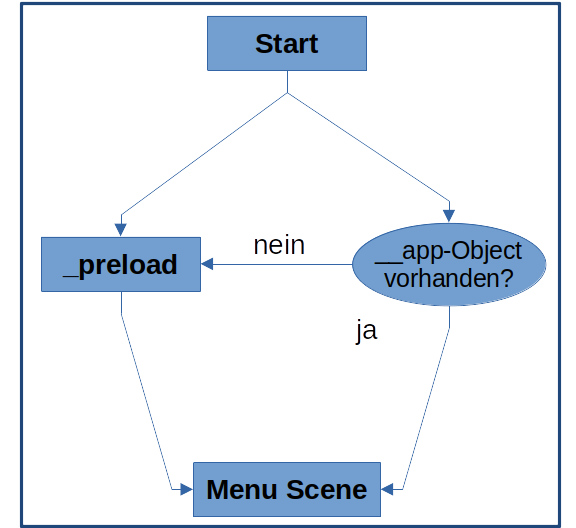
\includegraphics[width=.65\linewidth]{img/basic_start}
	\caption[structure]{Ablauf des Programmstarts}
	\label{fig:basic_start}
\end{figure}
%
\pagebreak
%
\section{Aufbau der Scenes}
\label{sec:scenestruct}
%
Jede Scene verfügt über ein oder mehrere eigene Controller Scripte, das die wichtigsten Funktionen steuern und, falls erforderlich, weitere Scripte aufrufen.
%
\begin{itemize}
	\item \pres{} \rarr \dls{} \& \sss{}
	\begin{itemize}
		\item \dls{}
		\begin{itemize}
			\item stellt alle erforderlichen Dateipfade zusammen
			\item lädt Einstellung aus \emph{settings.json}
			\item je nach Einstellung wird linke oder rechte Seite geladen
			\item Array für zu ladende Fahrzeugeinträge wird erstellen
			\item für jeden Fahrzeug-Array-Eintrag wird eine neue Instanz der \emph{Vehicle}-Class erzeugt und bekommt die jeweils geladenen Fahrzeugdaten zugewiesen
		\end{itemize}
		\item \ssc{}
		\begin{itemize}
			\item Zwischenspeicher für Status-Werte der aktuellen Session
			\item gespeichert werden:\\
			ausgewählte Sprache, gewählte Seite, Index der aktiven Scene und das gerade ausgewählte Fahrzeug 
		\end{itemize}
	\end{itemize}
	\item \mms{} \rarr \mss{}
	\begin{itemize}
		\item \msco{} zugeordnet
		\item Index für aktuelle Scene setzen
		\item Laden aller erforderlichen Elemente (Bild/Text) für die Darstellung des Auswahlmenüs
		\item Zuweisung der jeweiligen Button-Funktion
		\item Bei Auswahl einer Fahrzeugs \rarr Index des gewählten Fahrzeugs im \sss{} aktualisieren
	\end{itemize}
	\item \vhs{} \rarr{} \vehss
	\begin{itemize}
		\item Index für aktuelle Scene setzen
		\item Anzahl der verfügbaren Galerie-Bilder ermitteln
		\item alle verfügbaren Text-Informationen zum Fahrzeug einfügen
		\item verfügbare Galerie-Bilder laden
		\item zugehöriges 3D-Model aus den Prefabs laden
		\item alle zusätzlichen Button zunächst ausblenden
	\end{itemize}
\end{itemize}
%
\section{Programmstart}
\label{sec:app_start}
%
Das Ziel ist es bei jedem Programmstart, zunächst die \pres{} aufzurufen. Unabhängig davon, von welcher Scene aus gestartet wurde. Aus diesem Grund wird im \mss{} eine \am{} eingesetzt. Diese Methode läuft direkt nach dem \enquote{Erwachen} des Scripts und damit noch bevor die Inhalt in die Szene geladen werden. Wie in Zeile 4 \ref{lst:msas} zu sehen ist, wird hier die Methode \emph{sceneLoader.CheckPreLoadScene()} zu erst aufgerufen. Diese Methode ist Teil des \sls s, von dem aus sämtliche Scene-Übergänge gesteuert werden. In diesem Fall wird geprüft, ob in der Hierarchy bereits ein Object mit dem Namen \enquote{\_\_app} existiert. Sollte das nicht der Fall sein, wurde die \pres{} noch nicht geladen entsprechend ruft das \sls{} in Zeile 5 \ref{lst:cpls} die \pres{} auf.
%
\lstinputlisting[language={[Sharp]C},
caption={Jede Scene führt als erstes, CheckPreloadScene() aus.}, firstline=23, lastline=28, label={lst:msas}] {../../Assets/Scripts/MenuScene.cs}
%
\lstinputlisting[language={[Sharp]C},
caption={Sollte das \emph{\_\_app}-Object in der aktuellen Scene nicht existieren, wird anschließend die Scene \enquote{0} bzw. die \pres{} geladen.}, firstline=22, lastline=27, label={lst:cpls}] {../../Assets/Scripts/SceneLoader.cs}
%
\pagebreak
%
\section{Ladevorgang}
\label{sec:loading}
%
Das zuvor erwähnte \enquote{\_\_app}-Object beinhaltet das \dls{} und das \sss{}, beide werden während des Starts der \pres{} ausgeführt. Das \dls{} lädt innerhalb seiner \am{} zunächst die Settings-Datei (Zeile 5) \ref{lst:loadscript} und erzeugt anschließend ein Array der zu ladenden Fahrzeuge (Zeile 7). Im nächsten Schritt wird zusätzlich eine Liste der 3D-Modelle erstellt (Zeile 8). Um einen Error bei Fehlenden Daten beim Start zu vermeiden, wird anschließend noch geprüft, ob mit den geladenen Daten überhaupt eine Fahrzeugliste erstellt werden kann (Zeile 9). Die Bilder werden zunächst unsortiert geladen und erst nachträglich sortiert. Für jeden Ladevorgang kommt eine Methode vom Typ \emph{IEnumerator} zum Einsatz, die die Verwendung des \emph{yield return}-Befehls ermöglicht. Auf diese Weise können die Bilder über mehrere CPU-Threads verteilt und damit schneller geladen werden. Der Nachteil besteht darin, dass die Reihenfolge an dieser Stelle nicht erhalten bleibt und nachträglich wiederhergestellt werden muss. Die \sm{} (Wird direkt nach der \am{} ausgeführt) startet deshalb als erstes einen Sortieralgorithmus, um die unsortiert geladenen Galeriebilder aufsteigend nummeriert neu zu ordnen (Zeile 5) \ref{lst:loaderstart}. Danach wird eine kurze Ladepause ausgeführt. An dieser Stelle wäre es deutlich sinnvoller eine Methode zu verwenden, die auf das tatsächliche Ende einer \emph{yield return}-Befehls warten kann. Leider war diesem Zeitpunkt (Stand 04.08.21) keine Methode bekannt, die diese Funktion mitbringen würde. Zum Schluss wird das \sls{} aufgerufen und die nächste Scene, hier die \mms{} geladen (Zeile 11).
%
\lstinputlisting[language={[Sharp]C},
caption={Im \dls{} werden zunächst Arrays und Listen für die zu ladenenden Fahrzeugdaten erstellt und anschließend für jedes Fahrzeug instanziiert.}, firstline=55, lastline=66, label={lst:loadscript}] {../../Assets/Scripts/DataLoader.cs}
%
\pagebreak
%
\lstinputlisting[language={[Sharp]C},
caption={Durch den \emph{yield return}-Befehl kann der Ladevorgang über mehrere CPU-Threads verteilt werden und läuft damit schneller ab.}, firstline=214, lastline=231, label={lst:yieldreturn}] {../../Assets/Scripts/DataLoader.cs}
%
\lstinputlisting[language={[Sharp]C},
caption={In der \sm{} werden alle Galleriebilderlisten geordnet und nach einer kurzen ladepause in die nächste Scene gewechselt.}, firstline=262, lastline=274, label={lst:loaderstart}] {../../Assets/Scripts/DataLoader.cs}
%
\pagebreak
%
\section{Ablauf der \mms}
\label{sec:mms}
%
Wie unter \ref{sec:scenestruct} bereits erwähnt, wird innerhalb der \sm{} zunächst der Scene-Index aktualisiert (Zeile 3) \ref{lst:menustart}. Dann werden die Menü-Einträge der Fahrzeuge auf Basis der in \ref{sec:loading} geladenen Daten erstellt (Zeile 4). Innerhalb der \emph{CreateMenuEntries}-Methode wird dann für jedes geladenen Fahrzeug ein Button mit dem zugehören \emph{titlePic} des jeweiligen Fahrzeugs instanziiert (Zeile 6). Dann erhält der erstellte Button seine zugehörige \emph{Listener}-Funktion, die bei einem Klick ausgeführt werden sollen (Zeile 7). Anschließend werden noch Titel des Fahrzeugs und das jeweilige Erscheinungsjahr zugeordnet. Die Button werden an dieser Stelle auf Basis eines \emph{Prefabs} erzeugt, welches das Layout der Elemente vorgibt. Dieses \emph{Prefab} ist im \path{/Prefab/}-Verzeichnis unter dem Namen \enquote{MenuEntry} zu finden. 
%
\lstinputlisting[language={[Sharp]C},
caption={In der \sm{} des \mss{} wird als erstes der Scene-Index aktualisiert und anschließend werden die Menü-Einträge der Fahrzeuge erstellt.}, firstline=31, lastline=35, label={lst:menustart}] {../../Assets/Scripts/MenuScene.cs}
%
\lstinputlisting[language={[Sharp]C},
caption={An dieser Stelle wird für jedes geladenen Fahrzeug ein Button in der \mms{} erstellt.}, firstline=37, lastline=47, label={lst:menustart}] {../../Assets/Scripts/MenuScene.cs}
%
\pagebreak
%
\section{Ablauf der \vhs}
\label{sec:vhs}
%
Die \sm{} beginnt hier ebenfalls mit einer Aktualisierung des Scene-Index (Zeile 3) \ref{lst:vehiclestart}. Dann wird die Anzahl der Galeriebilder ermittelt (Zeile 7) und die Standard-Werte eingetragen (Zeile 8). Anschließend werden die Texte, Bilder und das 3D-Model den jeweiligen Elementen der GUI zugewiesen (Zeile 10-12). Außerdem werden die Booleans für das Starten der UI-Animationen auf den default-Wert \emph{false} gesetzt (Zeile 4-6). Dasselbe gilt für die Button, die nur im Zusammenhang mit animierten UI-Elementen angezeigt werden sollen (Zeile 13, 14). Die UI Animationen arbeiten auf Basis des Verschiebens der Objekte innerhalb der Hierarchy. Das bedeutet, dass immer die Elemente, die im Vordergrund stehen zuletzt gerendert werden bzw. unten in der Hierarchy stehen müssen, da diese von oben nach unten arbeitet. Diese Methode konnte bisher (Stand 04.08.21) noch nicht ausgiebig getestet werden und bringt das Risiko mit sich, dass teilweise nicht sichtbare Objekte über einem Button liegen könnten und ihn somit blockieren. Bisher (Stand 04.08.21) ist dieses Problem nur wenige mal aufgetreten und konnte jeweils auf einen Bug im Code zurückgeführt werden. Eine Besonderheit in der \vhs{} stellt das 3D-Model des Phänomen 4RL dar. Es ist bisher (Stand 04.08.21) das einzige 3D-Model, das über Animationen verfügt und benötigt deshalb einige zusätzliche Methoden und Abfragen. So werden beispielsweise die Abfragen zum Triggern der Animationen nur geladen, wenn die linke Seite aktiv ist und der Index des gewählten Fahrzeugs dem Wert in \emph{animModelArrayPos} entspricht. Eine ähnliche Abfrage findet sich außerdem im \ors{} (Zeile 3) \ref{lst:obrotstart} um zu prüfen, ob nach dem animierbaren 3D-Modellen gesucht werden soll oder nicht.
%
\lstinputlisting[language={[Sharp]C},
caption={Die \mms{} weist die Texte, Bilder und das 3D-Modell des ausgewählten Fahzeugs den jweiligen Layout-Elementen zu.}, firstline=69, lastline=83, label={lst:vehiclestart}] {../../Assets/Scripts/VehicleScene.cs}
%
\pagebreak
%
\lstinputlisting[language={[Sharp]C},
caption={Die Button zum Toggeln der Animationen werden nur gezeigt, wenn das Model des Phänomen 4RL auch ausgewählt ist.}, firstline=265, lastline=285, label={lst:vehiclecheck}] {../../Assets/Scripts/VehicleScene.cs}
%
\lstinputlisting[language={[Sharp]C},
caption={Hier wird im \ors{} geprüft, ob aktuell das Model des Phänomen 4RL geladen ist und somit anch den animierbaren Objekten gesucht werden soll oder nicht.}, firstline=22, lastline=34, label={lst:obrotstart}] {../../Assets/Scripts/ObjectRotation.cs}
%
\pagebreak
%
\section{Timer}
\label{sec:timer}
%
Die \emph{Timer}-Class hat die Aufgabe die \vhs{} in die \mms{} zurückzusetzen unter der Bedingung, dass über eine bestimmte Zeit keinerlei Eingaben erfolgt sind. Der Wert wird in die \emph{Settings}-Datei (\path{/StreamingAssets/Settings.json}) geschrieben und setzt sich aus dem \emph{invisibleCountdown} und dem \emph{visibleCountdown} Wert zusammen. Der \emph{invisibleCountdown} ist die Anzahl an Sekunden, die vergehen müssen, bevor auf dem Display der Reset-Timer angezeigt wird. sobald diese \enquote{nicht sichtbaren} Sekunden abgelaufen sind, werden die verbleiben \enquote{sichtbaren Sekunden angezeigt} (Zeile  9ff.) \ref{lst:disptime}. Dieser Wert entspricht der Angabe unter \emph{visibleCountdown} in der \emph{Settings.json} Datei. Der Countdown läuft damit im Hintergrund des \vhc{} ab und wird nur unter den angegebenen Bedingungen sichtbar. Um den Countdown bei jeder Interaktion mit der Oberfläche zurückzusetzen, steht \emph{ResetTimer} als einzige \emph{public methode} dieser Klasse zur Verfügung. Sie wird von jedem Button, jeder Zoom-/Scroll-Bar, den Rotationseingaben in der 3D-Vollbildansicht sowie den 3D-Animationen aufgerufen, um den Timer bei jeder Eingabe zurückzusetzen (Zeile 3) \ref{lst:resettime}.
%
\lstinputlisting[language={[Sharp]C},
caption={Sobald der im Hintergrund laufende \emph{displayTimeValue} den Rückgabewert von \emph{GetStateVisibleCountdown()} unterschritten hat, werden die Zahl des Countdowns auf dem Display angezeigt.}, firstline=16, lastline=34, label={lst:disptime}] {../../Assets/Scripts/Timer.cs}
%
\lstinputlisting[language={[Sharp]C},
caption={\emph{ResetTimer()} setzt den Timer auf seinen urspünglich geladenen Wert zurück.}, firstline=44, lastline=47, label={lst:resettime}] {../../Assets/Scripts/Timer.cs}